\documentclass[border=10pt]{standalone}

\usepackage{tikz}
\usepackage{tikzsymbols}
\usetikzlibrary{calc,patterns,shapes.geometric}

\def\centerarc[#1](#2)(#3:#4:#5){\draw[#1] ($(#2)+({#5*cos(#3)},{#5*sin(#3)})$) arc (#3:#4:#5);}

\begin{document}
	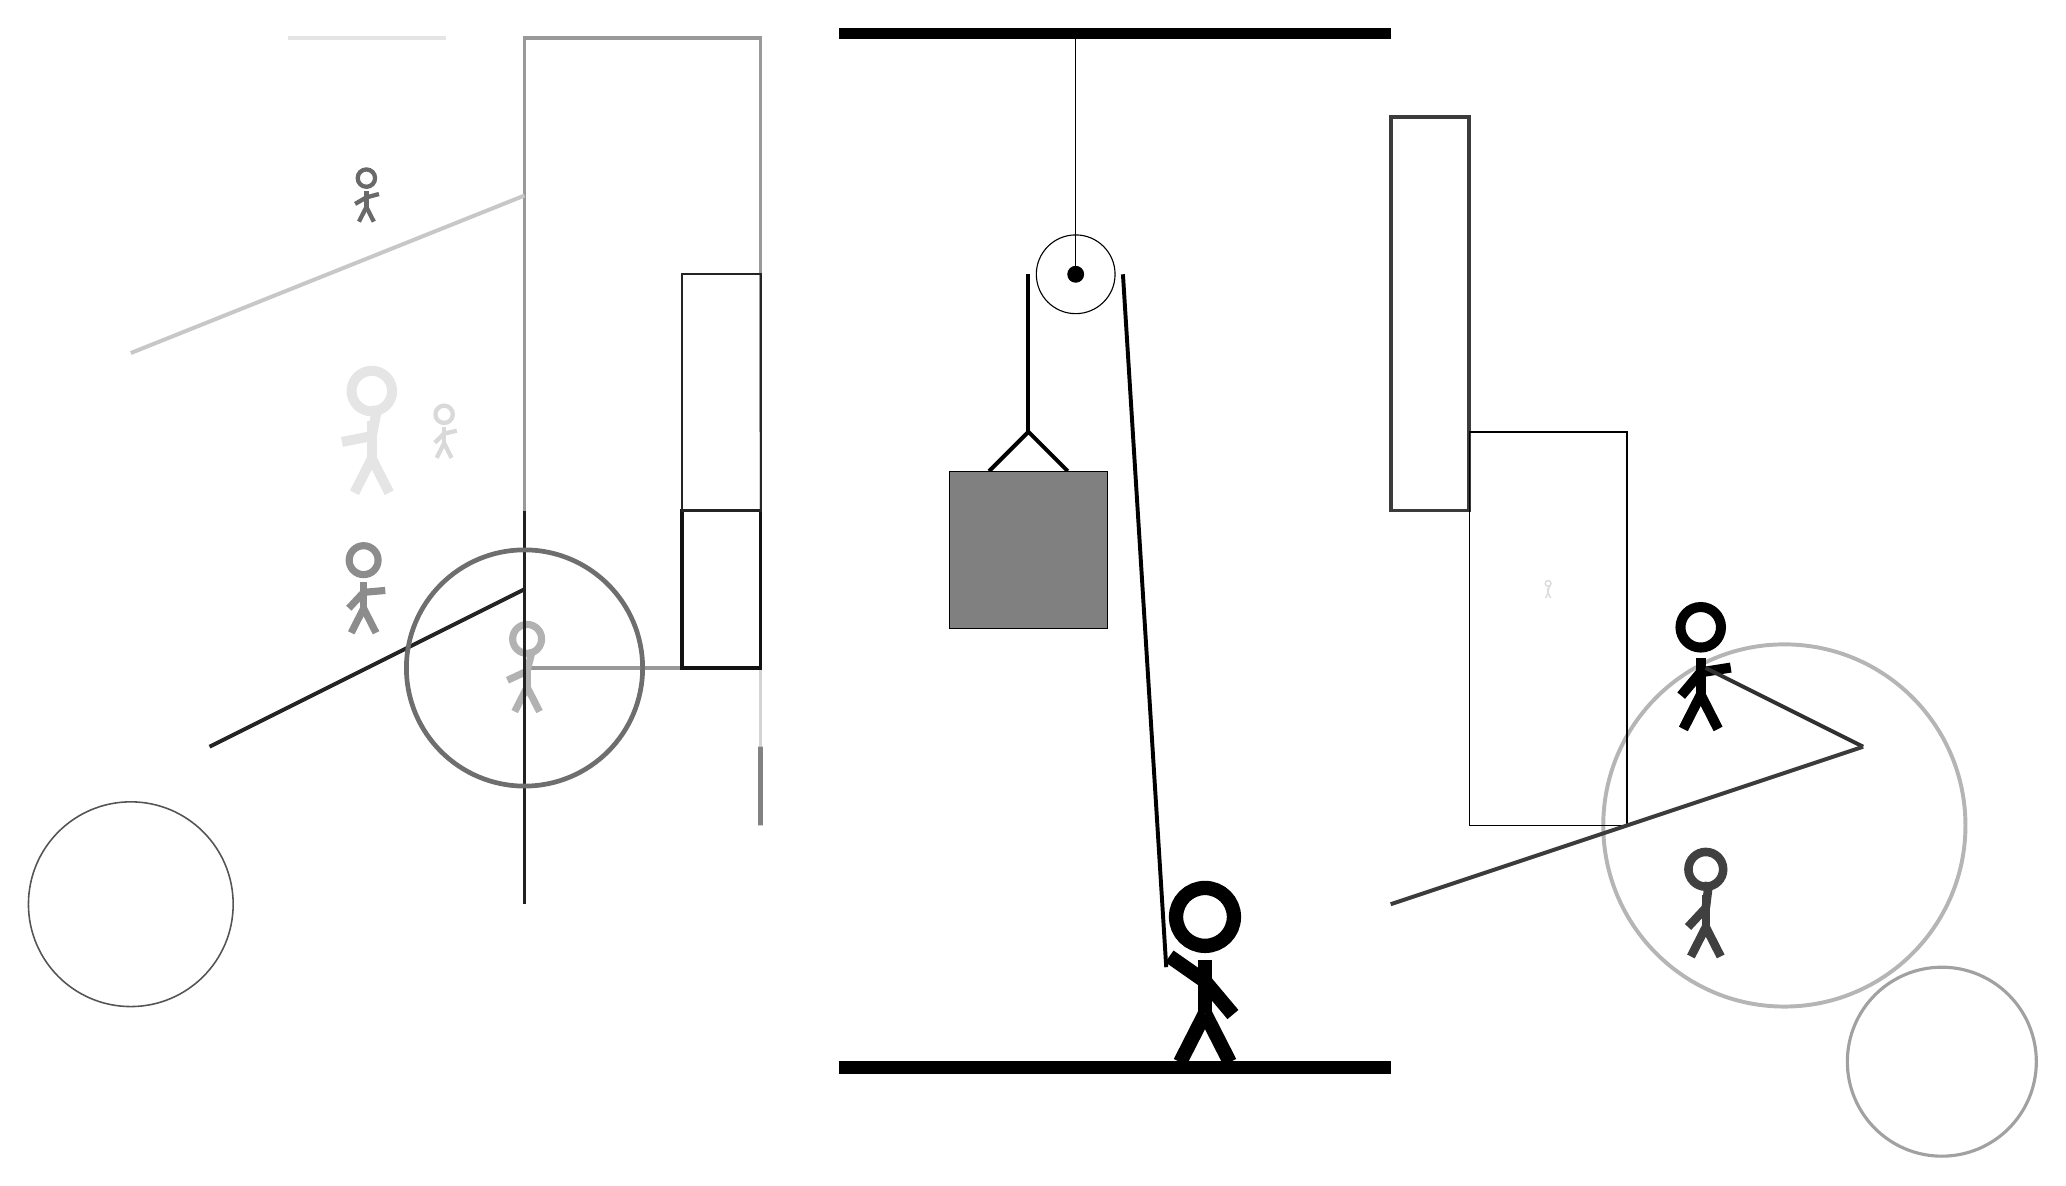
\begin{tikzpicture}
		%%%%% START %%%%%
		
		\draw[fill=black] (-2, 10) rectangle (5, 10.125);
		
		\draw (1, 7) circle (0.5);
		\draw[fill=black] (1, 7) circle (0.1);
		\draw (1, 10) -- (1, 7);
		
		\node[line width=0.3mm, color=black!59] at (-8, 8) {\Strichmaxerl[3][30][15]};
		
		\draw[line width=0.4mm, color=black!40] (-3, 2) rectangle (-6, 10);
		\draw[line width=0.5mm, color=black!86](-6, 3) -- (-10, 1);
		\node[line width=0.3mm, color=black!30] at (-6, 2) {\Strichmaxerl[5][25][76]};
		\draw[line width=0.5mm, color=black!10](-7, 10) -- (-9, 10);
		\draw[line width=0.4mm, color=black!17] (-3, 5) rectangle (-3, 1);
		\node[line width=0.7mm, color=black!75] at (9, -1) {\Strichmaxerl[6][47][83]};
		\draw [line width=0.5mm, color=black!29](10, 0) circle (2.3);
		\node[line width=0.2mm, color=black!10] at (-8, 5) {\Strichmaxerl[7][11][79]};
		
		\draw [line width=0.2mm, color=black!67](-11, -1) circle (1.3);
		\draw[line width=0.5mm, color=black!22](-6, 8) -- (-11, 6);
		\draw[line width=0.4mm, color=black!93] (-4, 4) rectangle (-3, 2);
		\draw[line width=0.7mm, color=black!49] (-3, 0) rectangle (-3, 1);
		
		\draw[line width=0.5mm, color=black!77] (5, 4) rectangle (6, 9);
		\draw[line width=0.5mm, color=black!87](-6, -1) -- (-6, 4);
		\node[line width=0.6mm, color=black!100] at (9, 2) {\Strichmaxerl[7][50][9]};
		\draw [line width=0.6mm, color=black!57](-6, 2) circle (1.5);
		\draw[line width=0.2mm, color=black!100] (6, 0) rectangle (8, 5);
		\draw[line width=0.3mm, color=black!86] (-3, 4) rectangle (-4, 7);
		
		\node[line width=0.6mm, color=black!45] at (-8, 3) {\Strichmaxerl[5][47][5]};
		\draw[line width=0.5mm, color=black!81](9, 2) -- (11, 1);
		
		\node[line width=0.6mm, color=black!15] at (-7, 5) {\Strichmaxerl[3][44][13]};
		\node[line width=0.2mm, color=black!14] at (7, 3) {\Strichmaxerl[1][88][67]};
		\draw [line width=0.4mm, color=black!37](12, -3) circle (1.2);
		\draw[line width=0.5mm, color=black!77](5, -1) -- (11, 1);
		
		\draw[line width=0.5mm] (-0.1, 4.5) -- (0.4, 5.0) -- (0.9, 4.5);
		\draw[fill=black!50] (-0.6, 4.5) rectangle (1.4, 2.5);
		
		\draw[line width=0.5mm] (0.4, 7) -- (0.4, 5.0);
		\centerarc[line width=0.5mm](1, 7)(0:180:0.6);
		\draw[line width=0.5mm](1.6, 7) -- (2.15, -1.8);
		
		\node at (2.6, -1.9) {\Strichmaxerl[10][-35][-50]};
		
		\draw[fill=black] (-2, -3) rectangle (5, -3.15);
		
		%%%%% END %%%%%
	\end{tikzpicture}
\end{document}